\graphicspath{{./images/chap3/}}
% Relevance Feedback
% Methodology
% * Design and Architecture
% * Population of interest and sampling subject used in the study
% * Instrument and what it measures (matrices)
% * qualifications of informants if used in the study
% * Validation
% * Data gathering procedure (experiments)
\chapter{Datasets} % (fold)
\label{cha:datasets}

All the experiments in this study are conducted on a database two species of
skinks: \emph{Grand} and \emph{Otago} of 3687 images in total created by
biologists at New Zealand Department of Conservation. 

\begin{figure}[ht]
  \centering
  \subfloat{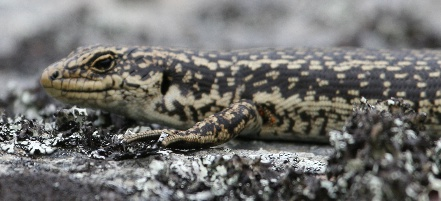
\includegraphics[width=4cm]{dataset/general/grand_L3}}
  \subfloat{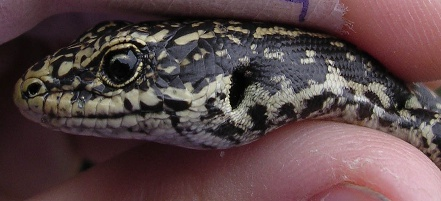
\includegraphics[width=4cm]{dataset/general/grand_L1}}
  \subfloat{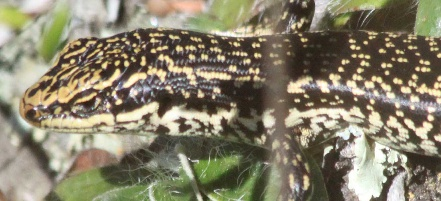
\includegraphics[width=4cm]{dataset/general/grand_L2}}\\

  \subfloat{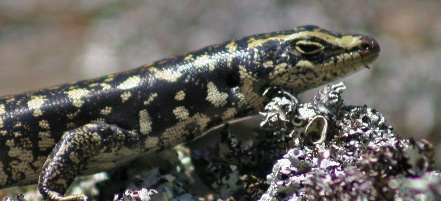
\includegraphics[width=4cm]{dataset/general/otago_R2}}
  \subfloat{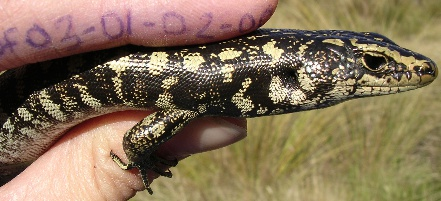
\includegraphics[width=4cm]{dataset/general/otago_R1}}
  \subfloat{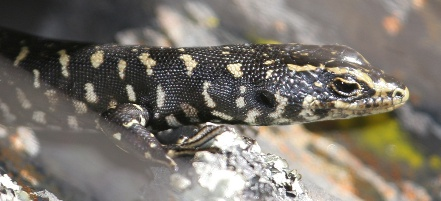
\includegraphics[width=4cm]{dataset/general/otago_R3}}\\
  \captionsetup{justification=centering}
  \caption{Top: Left view images from Grand dataset.\\Bottom: Right view images
  from the Otago dataset}
\end{figure}

The Grand database contains 1871 \texttt{RGB} images of 206 individuals with
variations in sizes, lighting, and background, while the Otago database
contains 1816 \texttt{RGB} images of 221 individuals, also with such
variations. The images are closely cropped to include only the anterior end of
the subjects; therefore, the size varies from 1056 $\times$ 564 to 2437
$\times$ 1215 pixels

\begin{table}[t]
\captionsetup{justification=centering}
  \caption{Summary of each database}
  \label{database-table} %chktex 24
  \centering
  \begin{tabular}{lccccccc}
    \toprule
    & \multicolumn{3}{c}{Number of Images} & & &
        \multicolumn{2}{c}{Images per Individual} \\
    \cmidrule{2-4}
    \cmidrule{7-8}
    Name & Left View & Right View & Total & Individuals & Singletons & Avg.
        & Max. \\
    \midrule
    Grand & 929 & 942 & 1871 & 206  & 69 & 9 & 31 \\
    Otago & 903 & 913 & 1816 & 221  & 58 & 8 & 24 \\
    \bottomrule
  \end{tabular}
\end{table}


\section{General}

\subsection{Selfscore and Score Distributions}

Sloop ranks the likelihood that two capture events contain the same individuals
quantitatively by a score. The similarity score between two individuals is
obtained from comparing sift features of all the images within a capture
capture to sift features of the images within the other individual's cohort
\emph{normalized by the minimum selfscore among all the images in the
comparison}. A capture is a group of images containing the same individual, not
necessarily having the same view, that is captured together, whereas a cohort
is a group of images that are identified as the same animal, not necessarily
having the same view or captured at the same time.

\subsubsection{Selfscores}

Selfscore of a capture is the \emph{maximum} selfscore of all the images within
the capture, where a selfscore of an image is calculated from comparing the
sift features of each image with itself.  $$\texttt{selfscore}(C) =
\max_{\forall I_i \in C} \texttt{sift\_match}(I_i, I_i)$$ 

\begin{figure}[h!]
  \centering
  \subfloat[Selfscores]{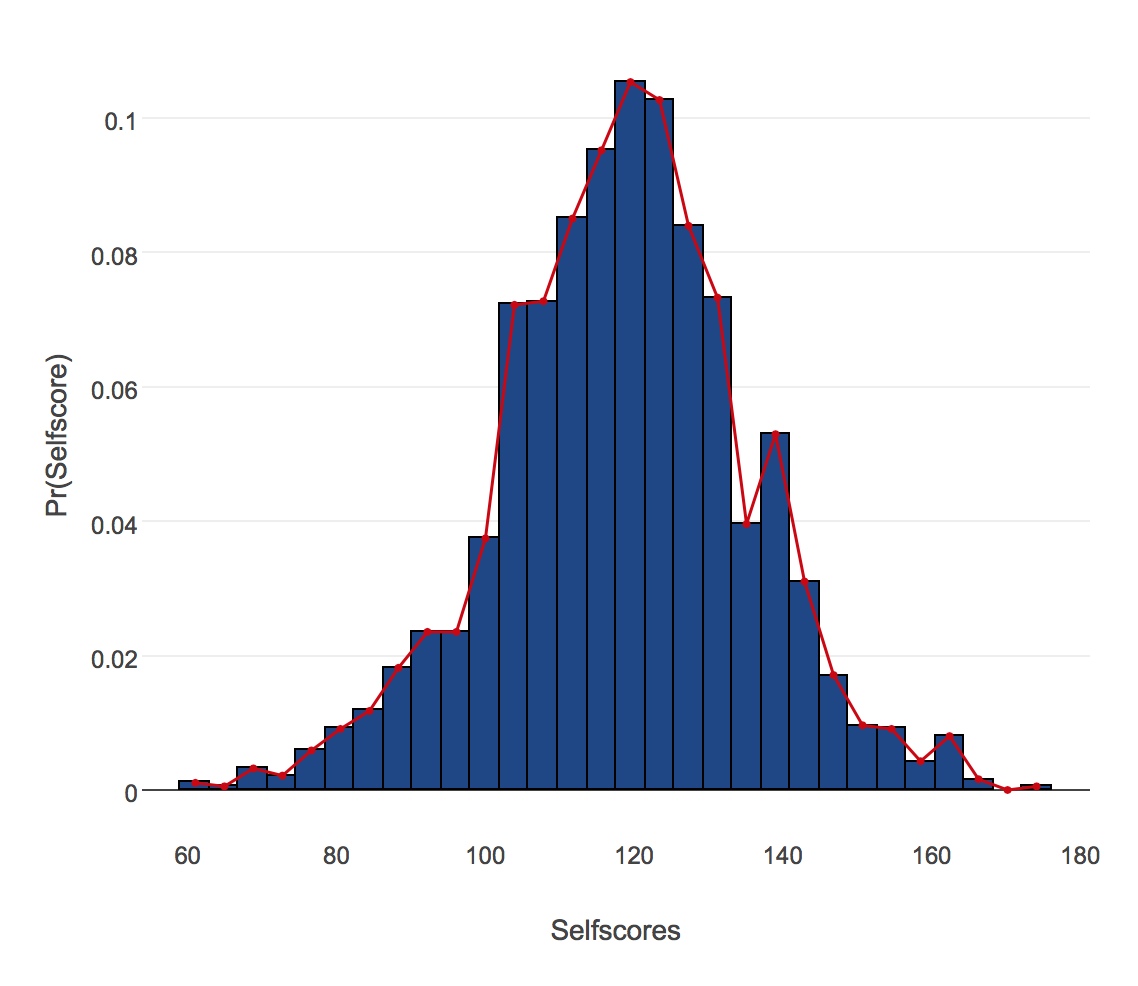
\includegraphics[width=0.58\textwidth]
      {dataset/grand/selfscores}}\qquad
  \subfloat[CDF of selfscores]{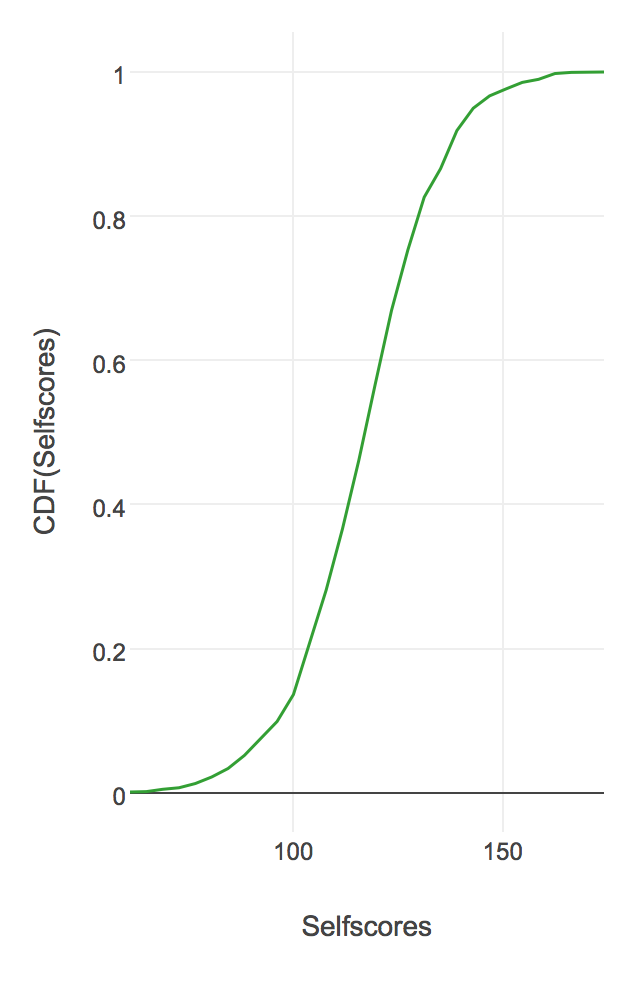
\includegraphics[width=0.3\textwidth]
      {dataset/grand/cdf_selfscores}}
  \captionsetup{justification=centering}
  \caption{Selfscore Distribution}
\end{figure}

\begin{figure}[h!]
  \centering
  \subfloat[Selfscores]{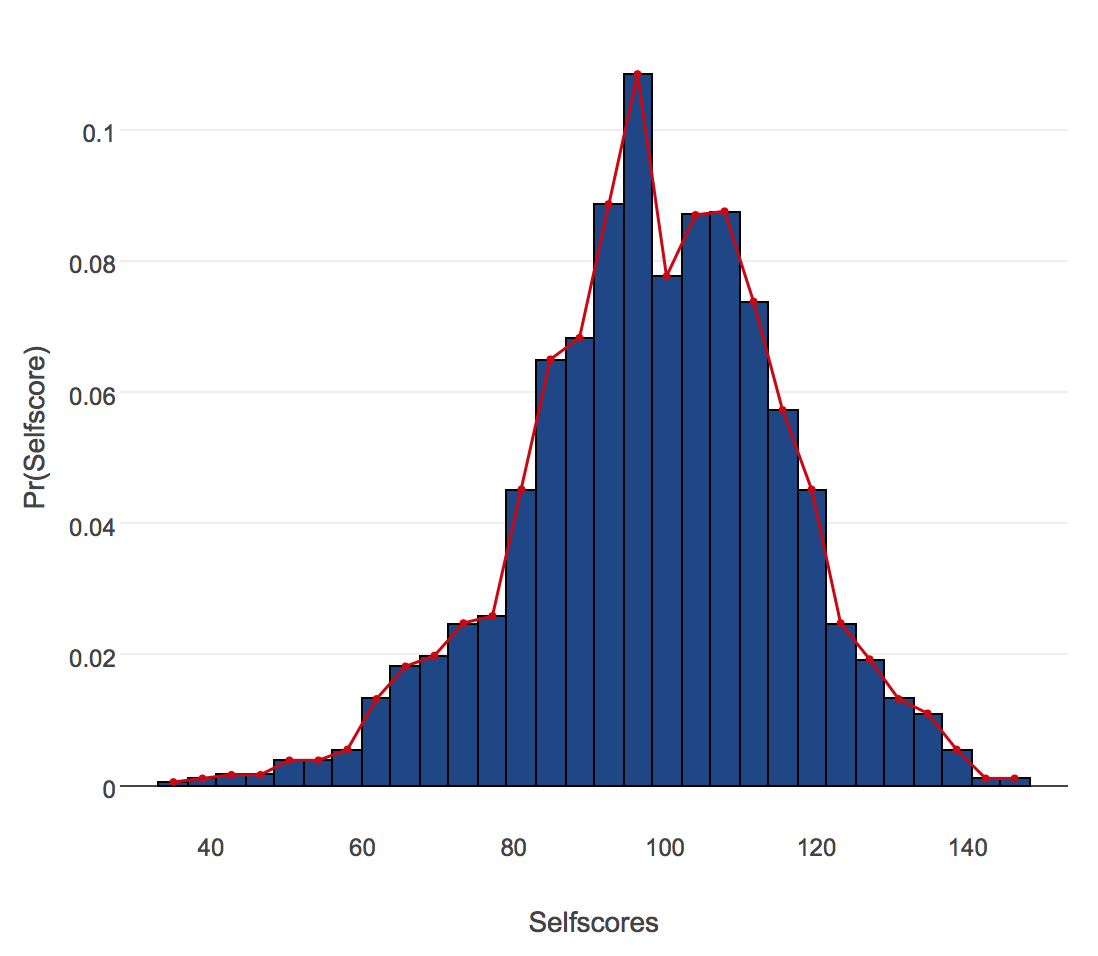
\includegraphics[width=0.58\textwidth]
        {dataset/otago/selfscores}}\qquad
  \subfloat[CDF of selfscores]{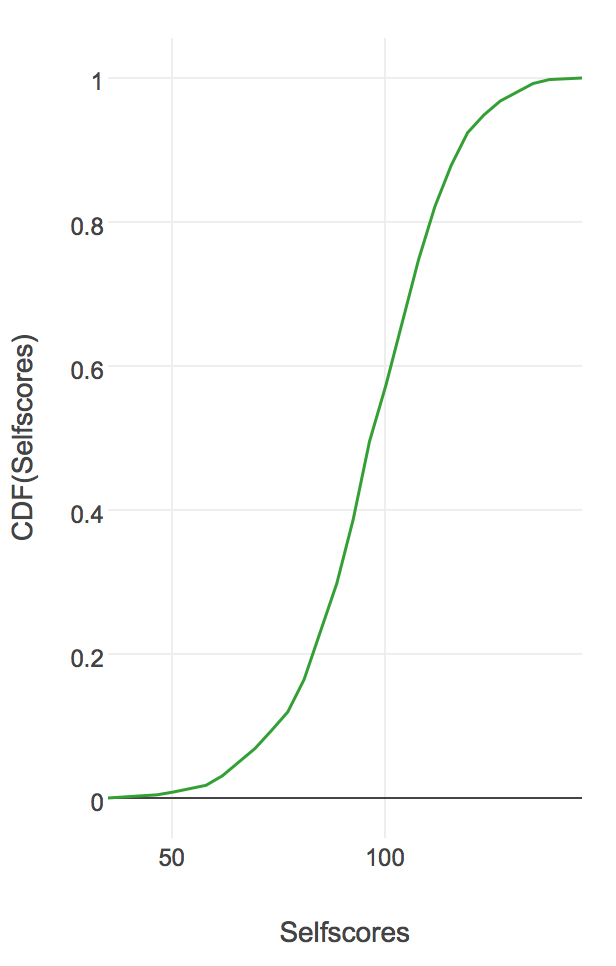
\includegraphics[width=0.3\textwidth]
        {dataset/otago/cdf_selfscores}}
  \captionsetup{justification=centering}
  \caption{Selfscore Distribution}
\end{figure}

\subsubsection{Scores}

The score between the two individuals is the maximum score among all the
comparisons among the images within the cohorts.

$$\texttt{score}(C_1, C_2) = \max_{\forall I_i \in C_1 \forall I_j \in C_2}
    \frac{\texttt{sift\_match}(I_i, I_j)}{\min(\texttt{selfscore}(C_1),
        \texttt{selfscore}(C_2))}$$
where $C$ is a capture and $I$ is an image in a capture.

\begin{figure}[ht]
  \centering
  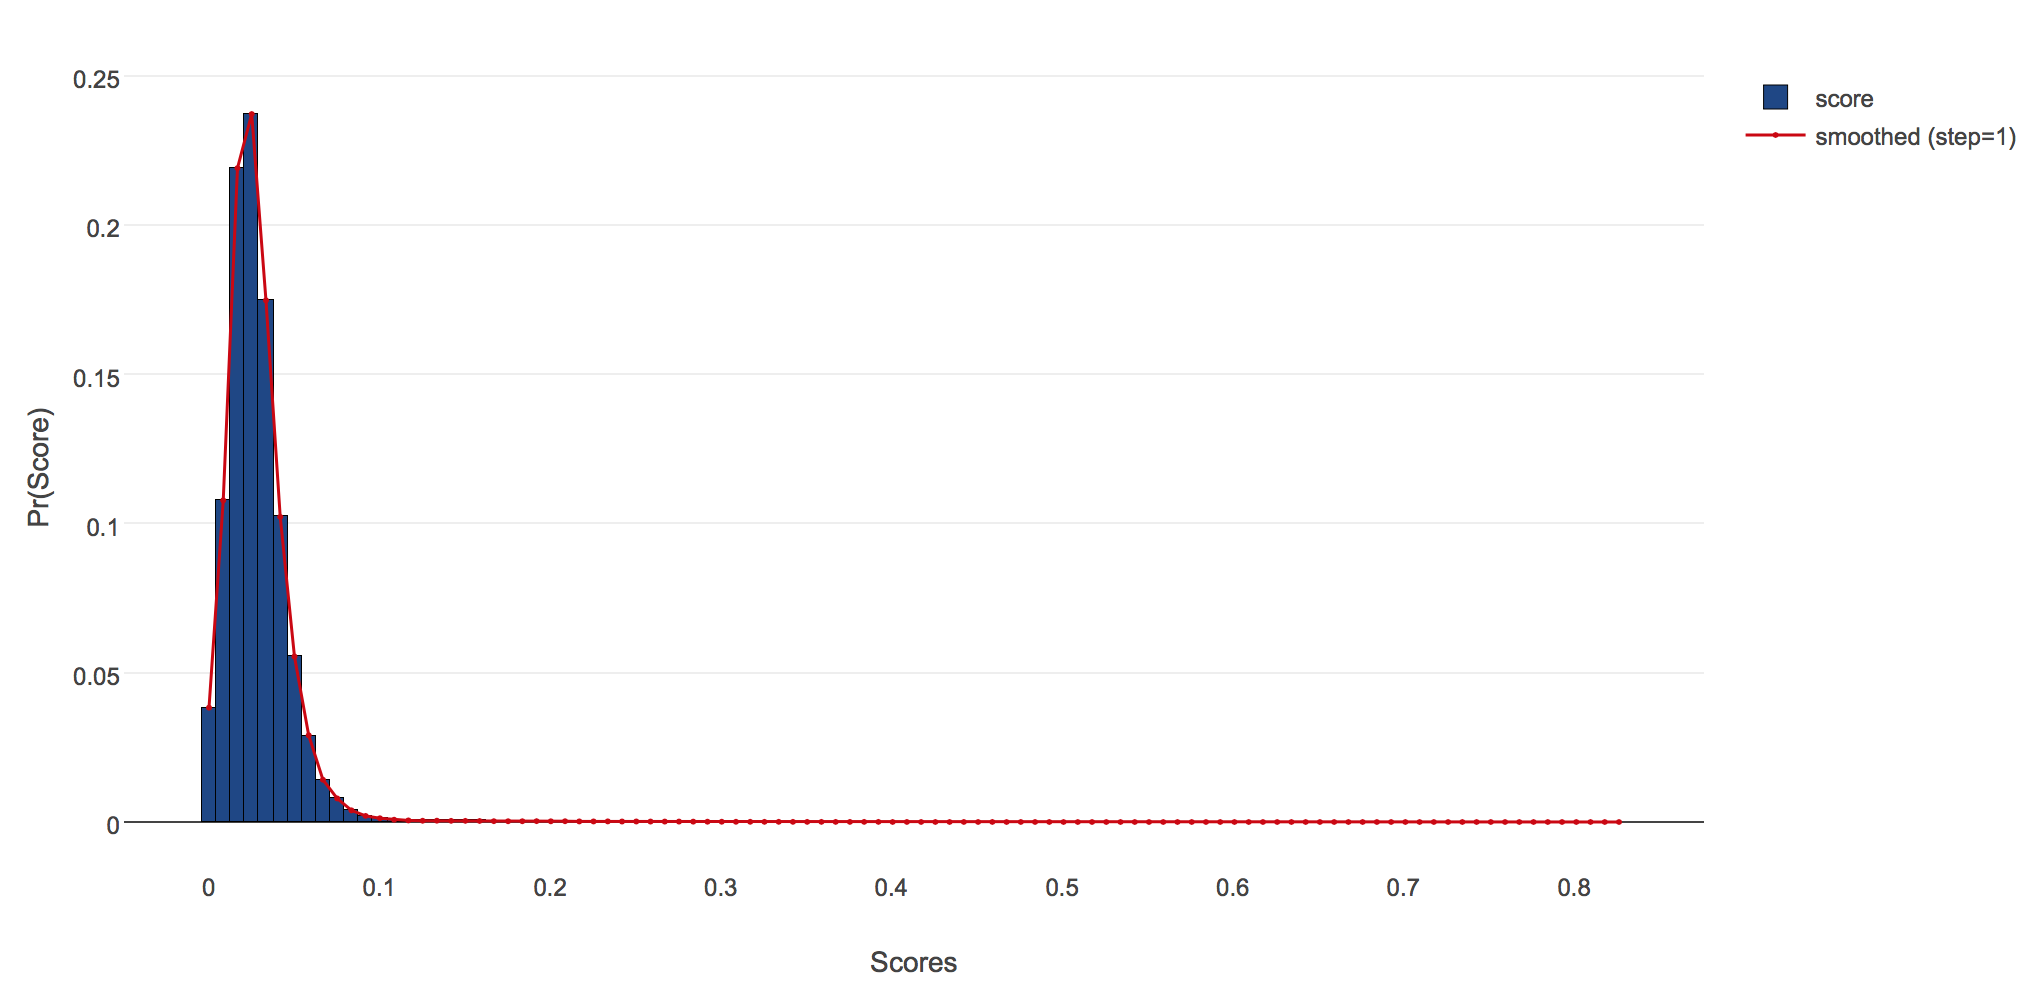
\includegraphics[width=\textwidth]{dataset/grand/scores}
  \caption{Score Distribution}
  \label{fig:grand_scores} %chktex 24
\end{figure}

\begin{figure}[ht]
  \centering
  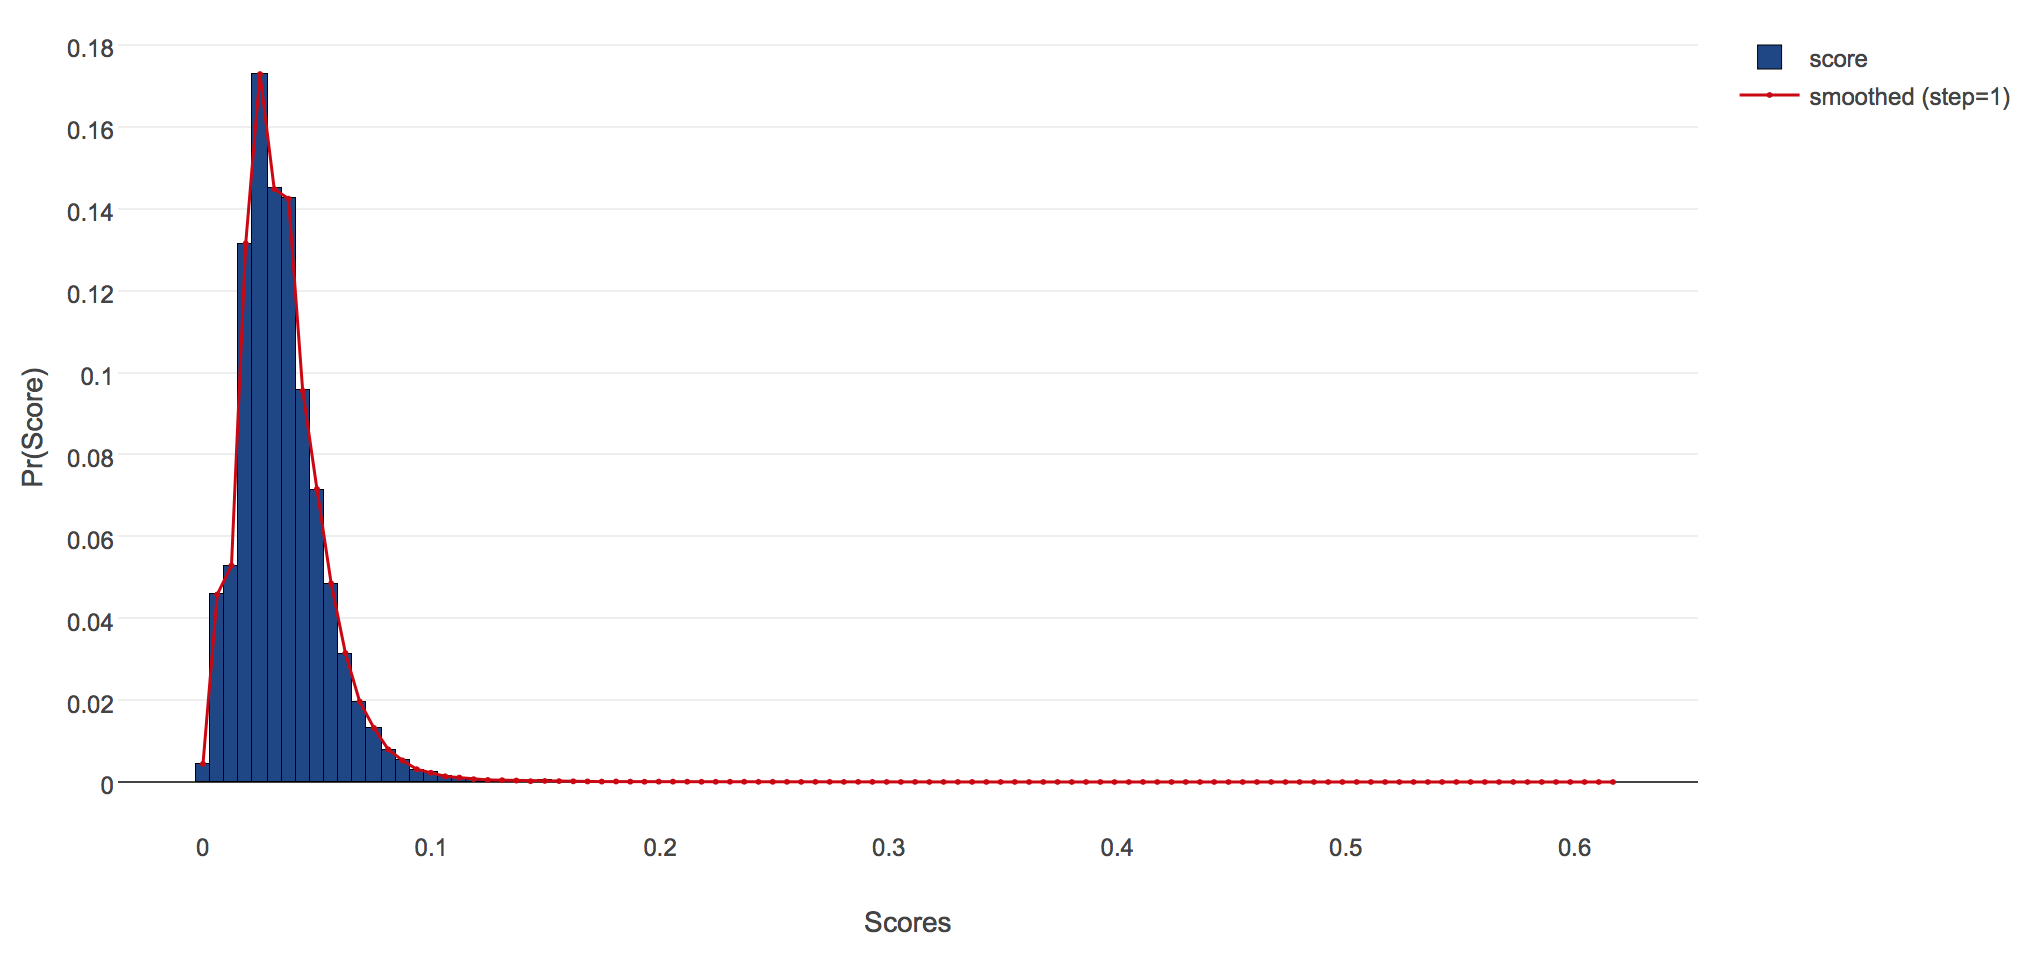
\includegraphics[width=\textwidth]{dataset/otago/scores}
  \caption{Score Distribution}
  \label{fig:otago_scores} %chktex 24
\end{figure}
